\documentclass[11pt,a4paper]{article}
\usepackage[margin=23mm]{geometry}
\usepackage[T1]{fontenc}
\usepackage{lmodern}
\usepackage{hyperref}
\usepackage{tikz}
\usetikzlibrary{positioning,arrows.meta}
\title{Core distributed semantics: specification and formal verification}
\date{Created-at: 2026-09-05 17:10 CEST}
\begin{document}
\maketitle
\paragraph{Scope.}
Continue the user's distributed execution investigation, update its existing
single-writer/replica semantics, and verify concrete safety properties. This
does not imply multi-writer consensus, an implemented scheduler, or unrestricted
algebraic reassociation. The earlier dependency/CI, browser and consumer stages
remain in scope for subsequent integration; Amaterasu is authorized.
\paragraph{ETA.}
45--90 minutes: public-API counterexamples, a small Lean model using the
already installed 4.19.0 toolchain, specification corrections, traceability,
review and report. Individual verification commands are bounded and logged.
\paragraph{Source and ownership.}
Own Core worktree D:/hnnwork/distributed/core, branch
audit/core-distributed-semantics-2026-09-05, base 4a243ede85b7dd1f488bc9c68a46086a8638e39c.
Core owns the IR, portable codec, version tuple and transaction assembler.
Chordex owns opaque transport. Consumers own computation scheduling and
installation, with domain algorithms in their existing framework owners.
The existing Core specification and docs/verification/unified-ir remain the
canonical location. The historical proofs directory is empty; unrelated
SymPy/Z3 algebra proofs are not evidence of distributed replay correctness.
\paragraph{Discovery.}
Read unified-ir-architecture Part G, hypergraph-synchronization, requirements,
SnapshotVersion, TransactionAssembler and existing test scaffolding. Reuse the
public EnvelopeDraft/encode/validate/apply boundary. Do not duplicate assembler
or IR code in a worker. Lean will model only the commit admission boundary,
with explicitly stated abstraction and refinement limits.
\paragraph{Files.}
Modify docs/unified-ir-architecture.md, docs/hypergraph-synchronization.md and
docs/verification/unified-ir/requirements.md. New:
docs/verification/unified-ir/distributed-semantics.lean;
docs/plans/2026-09-05-distributed-semantics/plan.tex, plan.pdf, plan.tikz, plan.mmd;
reports/2026-09-05-distributed-semantics.md and
reports/distributed-semantics/ (Rust probe, logs, traceability and hashes).
Extend .gitattributes only for exact evidence bytes. No new Cargo dependency.
\paragraph{Protected changes.}
Initial protected Core source edits: empty list. First reproduce admission
gaps through the public facade and prepare a concrete minimal correction with
regression/rollback details. The Core manifest requires a scoped token for a
protected implementation edit; existing Graph approvals do not name this code.
Independent specification and proof work proceeds without such edits.
\paragraph{Verification.}
Check version-order laws, non-regression, equal-version unknown-identity
rejection, stale delta rejection, replay identity, and conditional replica
convergence. Kernel-check Lean theorems without sorry or added axioms; record
their actual axiom dependencies. A proof about the abstract model is not a
proof of Rust refinement, payload validation, durable crash recovery or liveness.
Run an independent Rust probe against the exact containerized Core on Amaterasu;
include negative controls that expose implementation violations rather than
changing expected outcomes to obtain a green acceptance result.
\paragraph{Budgets and risks.}
At most 16 GiB RSS, no swap/virtual-memory cap. Remote probes use the existing
bounded Docker SDK, network disabled. Lean uses the existing 2 GiB sampled RSS
guard; no package download. The installed 4.19.0 rejects the attempted internal
memory option, so that failed attempt is retained rather than counted as a cap.
Capture exit, wall
time and RSS; sample-based RSS limits are not a kernel quota. No throughput
claim from tiny probes. Risks include missing persisted identities, incomparable
version tuples, payload-vs-structural-hash confusion, and unsupported claims of
exactly-once work or atomic installation from transport receipt alone.
\paragraph{Acceptance and rollback.}
Every requirement separates normative model proof from observed runtime status.
Preserve and report any red runtime acceptance check. Keep the prior audit and
Docker evidence unchanged. Local thematic commits are authorized by the
continuing task; no push, merge, release or global host changes. Roll back only
this branch's named changes, retaining failure evidence needed for review.
\begin{center}
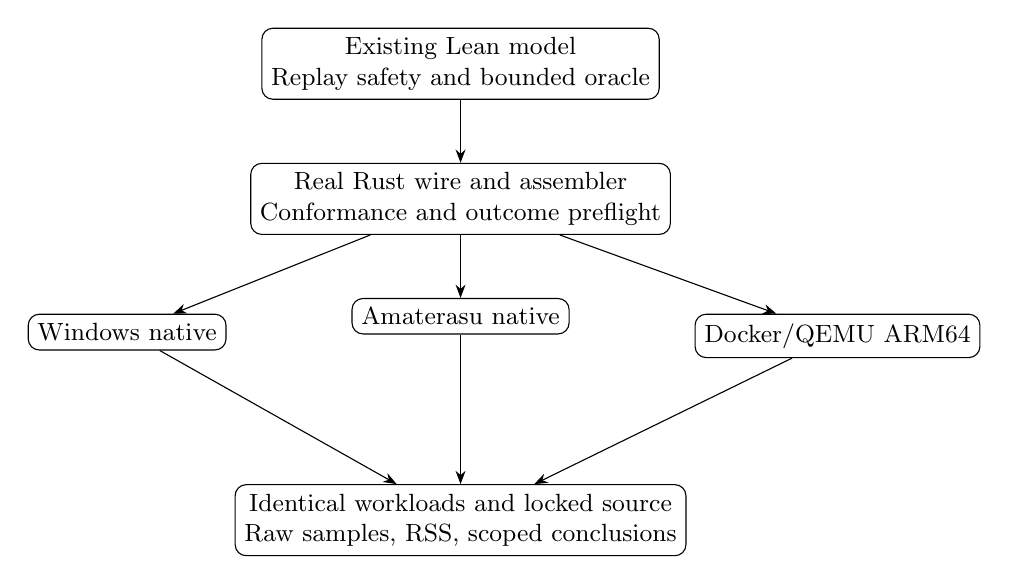
\begin{tikzpicture}[node distance=8mm, every node/.style={draw,align=center,rounded corners,font=\small}, >=Stealth]
\node (model) {Existing Lean model\\Replay safety and bounded oracle};
\node[below=of model] (rust) {Real Rust wire and assembler\\Conformance and outcome preflight};
\node[below left=10mm and 3mm of rust] (local) {Windows native};
\node[below=of rust] (linux) {Amaterasu native};
\node[below right=10mm and 3mm of rust] (arm) {Docker/QEMU ARM64};
\node[below=19mm of linux] (report) {Identical workloads and locked source\\Raw samples, RSS, scoped conclusions};
\draw[->] (model)--(rust); \draw[->] (rust)--(local); \draw[->] (rust)--(linux); \draw[->] (rust)--(arm);
\draw[->] (local)--(report); \draw[->] (linux)--(report); \draw[->] (arm)--(report);
\end{tikzpicture}
\end{center}

\end{document}
